\documentclass[12pt]{article}
\usepackage[utf8]{inputenc}
\usepackage{amssymb}
\usepackage{amsmath,amsthm}
\usepackage{tikz}
\usetikzlibrary{arrows,decorations.markings, matrix}
\tikzset{->-/.style={decoration={
              markings,
              mark=at position .5 with {\arrow{>}}},postaction={decorate}}}
\tikzset{-<-/.style={decoration={
              markings,
              mark=at position .5 with {\arrow{<}}},postaction={decorate}}}
\usetikzlibrary{shapes.multipart}
\usetikzlibrary{decorations.pathmorphing,shapes}
\usetikzlibrary{decorations.pathreplacing}

\newcommand{\Trop}{\OP{Trop}}

\newcommand{\OP}[1]{\mathrm{#1}}

\begin{document}

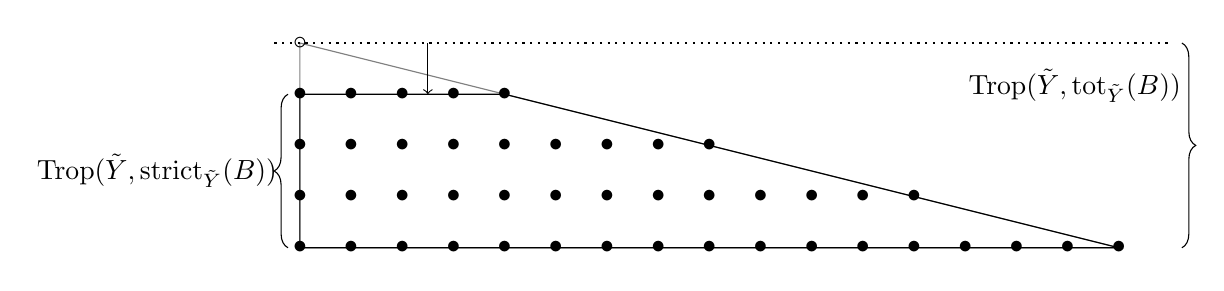
\begin{tikzpicture}[scale=0.65]
  \draw[draw=gray] (0,0) -- (16,0) -- (0,4) -- cycle;
  \foreach \x in {0,1,2,...,16} {\node at (\x,0) {\(\bullet\)};}
  \foreach \x in {0,1,...,12} {\node at (\x,1) {\(\bullet\)};}
  \foreach \x in {0,1,...,8} {\node at (\x,2) {\(\bullet\)};}
  \foreach \x in {0,1,...,4} {\node at (\x,3) {\(\bullet\)};}
  \foreach \x in {0} {\node at (\x,4) {\(\circ\)};}
  \draw (0,0) -- (16,0) -- (4,3) -- (0,3) -- cycle;
  \draw[dotted,thick] (-0.5,4) -- (17,4);
  \draw[->] (2.5,4) -- (2.5,3);
  \node at (-1,1.5) {};
  \draw [decorate,decoration={brace,amplitude=5pt,raise=1ex}] (0,0) -- (0,3) node[midway,xshift=-12ex]{\(\Trop(\tilde{Y},\OP{strict}_{\tilde{Y}}(B))\)};
  \draw [decorate,decoration={brace,amplitude=5pt,raise=1ex}] (17,4) -- (17,0) node[midway,xshift=-8ex,yshift=5ex]{\(\Trop(\tilde{Y},\OP{tot}_{\tilde{Y}}(B))\)};
\end{tikzpicture}

\end{document}